\documentclass[border=2mm]{standalone}
\usepackage{tikz}

\begin{document}
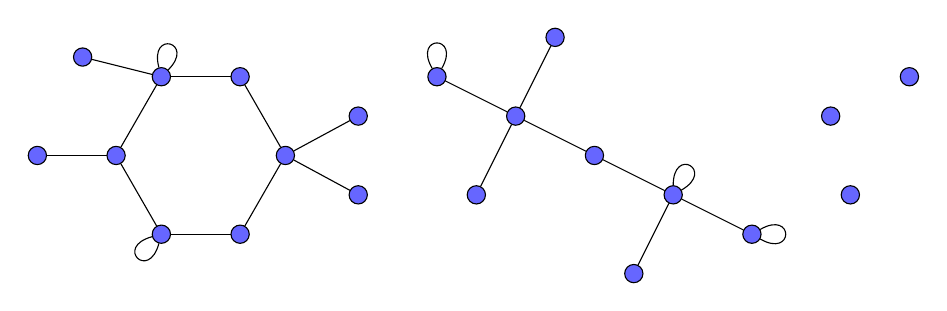
\begin{tikzpicture}[every node/.style={draw,circle,scale=0.7,fill=blue!60}]
  \node (0) at (-0.5, 1) {};
  \node (1) at (0.5, 1) {};
  \node (2) at (1.075, 0) {};
  \node (3) at (0.5, -1) {};
  \node (4) at (-0.5, -1) {};
  \node (5) at (-1.075, 0) {};
  \node (7) at (2, -0.5) {};
  \node (8) at (2, 0.5) {};
  \node (9) at (-1.5, 1.25) {};
  \node (10) at (3, 1) {};
  \node (11) at (4, 0.5) {};
  \node (12) at (5, 0) {};
  \node (13) at (6, -0.5) {};
  \node (14) at (7, -1) {};
  \node (15) at (4.5, 1.5) {};
  \node (16) at (3.5, -0.5) {};
  \node (17) at (5.5, -1.5) {};
  \node (18) at (-2.075, 0) {};
  \node (19) at (8.25, -0.5) {};
  \node (20) at (8, 0.5) {};
  \node (21) at (9, 1) {};
  \draw (0) to (1);
  \draw (1) to (2);
  \draw (2) to (3);
  \draw (3) to (4);
  \draw [in=-105, out=-165, loop] (4) to ();
  \draw (4) to (5);
  \draw (5) to (0);
  \draw (0) to (9);
  \draw (2) to (8);
  \draw (7) to (2);
  \draw [in=45, out=105, loop] (0) to ();
  \draw (10) to (11);
  \draw (12) to (11);
  \draw (12) to (13);
  \draw (13) to (14);
  \draw (15) to (11);
  \draw (11) to (16);
  \draw (17) to (13);
  \draw [in=30, out=-30, loop] (14) to ();
  \draw [in=30, out=90, loop] (13) to ();
  \draw [in=60, out=120, loop] (10) to ();
  \draw (18) to (5);
\end{tikzpicture}
\end{document}
